\documentclass[12pt,twoside,openright]{article}
\usepackage[utf8]{inputenc}
\usepackage[T1]{fontenc}
\usepackage[english]{babel}
\usepackage[a4paper,width=150mm,top=25mm,bottom=25mm]{geometry}
\usepackage{graphicx}
\usepackage{verbatim}
\usepackage{rotating}
\usepackage{pdflscape}
\usepackage{afterpage}
\usepackage{booktabs}
\usepackage{tocloft}
\usepackage{ textcomp }
% lol chapter space
\usepackage{etoolbox}

% \setcounter{tocdepth}{3}

% loa, lol vertical spacing
\usepackage{setspace}
\usepackage{float}


% paragraph
\setlength{\parindent}{0em}
\setlength{\parskip}{1em}

% headers and footers
\usepackage{fancyhdr}
\pagestyle{fancy}

% common
\fancyhead{}
% \fancyhead[RO,LE]{\leftmark}
\fancyhead[RO,LE]{\rightmark}
\fancyfoot{}
\fancyfoot[LE,RO]{\thepage}
\renewcommand{\headrulewidth}{0.4pt}
\renewcommand{\footrulewidth}{0.4pt}

% layouts, chapters, etc.
\fancypagestyle{plain}{%
    \fancyhead{}
    \fancyfoot{}
    \fancyfoot[LE,RO]{\thepage}
    \renewcommand{\headrulewidth}{0pt}
    \renewcommand{\footrulewidth}{0.4pt}
}

% blank pages
\makeatletter
\def\cleardoublepage{\clearpage\if@twoside \ifodd\c@page\else
    \hbox{}
    \thispagestyle{empty}
    \newpage
    \if@twocolumn\hbox{}\newpage\fi\fi\fi}
\makeatother

% images
\usepackage{graphicx}
\graphicspath{ {images/} }
\usepackage{array}
\usepackage{caption}
\usepackage{subcaption}

% tables
\setlength{\arrayrulewidth}{0.15mm}
\setlength{\tabcolsep}{8pt}
\renewcommand{\arraystretch}{1.3}
\newcolumntype{M}[1]{>{\centering\arraybackslash}m{#1}}
\newcommand{\ra}[1]{\renewcommand{\arraystretch}{#1}}
% equations
\usepackage{amsmath}

% algorithms
% \usepackage{amsmath}
\usepackage{algorithm}
\usepackage{algpseudocode}


% appendix
\usepackage[toc,page]{appendix}

% bibliography
\usepackage[nottoc]{tocbibind}

% hyperlinks
\usepackage{hyperref}
\hypersetup{
    colorlinks=true,
    linkcolor=black,
    urlcolor=black,
    citecolor=black,
}

% content
% \usepackage{tocloft}
% \cftsetindents{section}{0.5in}{0.5in}
% \cftsetindents{subsection}{0.5in}{0.5in}
% \cftsetindents{subsubsection}{0.5in}{0.5in}
\usepackage{outlines}


\begin{document}

\pagenumbering{gobble}
\begin{titlepage}
    \begin{center}
        \vspace*{1cm}
        
        \huge
        \textbf{Explain variable influence in black box models through pattern mining}
        
        \vspace{2cm}
        
        \large
        Xiaoqi Ma \\
        \href{mailto:xiaoqi.ma@rwth-aachen.de}{xiaoqi.ma@rwth-aachen.de} \\
        Matriculation number: 383420

        \vspace{1cm}

        Supervisor: Prof. Dr. Markus Strohmaier \\
        Second Examiner: Prof. Dr. Bastian Leibe\\
        Advisor: Dr. Florian Lemmerich \\

        \vspace{1.5cm}

        Chair of Computational Social Sciences and Humanities \\
        RWTH Aachen Faculty of Mathematics, Computer Science and Natural Sciences \\
        RWTH Aachen University 
        
        \vfill
        
        This thesis is submitted for the degree of \\
        M.Sc. Media Informatics
        
        \vspace{3cm}
        
        Aachen, Germany \\
        December 10, 2019
        
        
    \end{center}
\end{titlepage}
\cleardoublepage

\pagenumbering{arabic}

%\thispagestyle{plain}
\topskip0pt
\vspace*{\fill}
\begin{center}
	\Large
	\textbf{Acknowledgements}
\end{center}

\vspace{1cm}


First, I would like to express my sincere gratitude to my supervisor Prof. Dr. Thomas Rose for the continuous support of my master thesis and research, for his patience, motivation, and immense knowledge, also my advisor Thomas Osterland for his insightful comments and encouragement, and last not least the second supervisor Prof. Prinz for his kindness and support. Their guidance helped me in all the time of research and writing of this thesis.
Second, I owe the success of my master study and this thesis to my parents, Jing Zhou and Ping Yang, and my boy friend, Meng Li. They supported me through the difficulties that I encountered during the work.
\vspace*{\fill}
%\cleardoublepage

%\thispagestyle{plain}
\topskip0pt
\vspace*{\fill}
\begin{center}
	\Large
	\textbf{Abstract}
\end{center}

\vspace{1cm}
Understanding the decisions made by machine learning models is crucial for decision-makers and end-users. Enforced by GDPR, "right to explanation" demands businesses to provide understandable justifications to their users. Thus, it is of paramount importance to elucidate the model decision, which could be measured by model interpretability, the degree to which a human can understand the cause of a decision. In order to interpret black-box models, model-agnostic approaches could be applied, which provide flexibility in the choice of models, explanations and representation for models. From global interpretability viewpoint, feature importance and global surrogate are going to be explored. We also investigate the local model-agnostic methods, like LIME and Shapley value. After obtaining the designated feature contribution for each instance, we could use the subgroup discovery technique to figure out "interesting" patterns to provide more elaborate explanations. In this thesis, the aim is to build up a python package to provide a collection of tools to explain variable influence in black-box models through subgroup discovery. 


	\textbf{Keywords}: \textit{Black box model interpretability; Model agnostic; Subgroup discovery}

\vspace*{\fill}
%\cleardoublepage

\tableofcontents
\newpage

\section{Introduction}
\pagenumbering{arabic}

Assume we had a scenario where an unemployed young wanted to get a loan from the bank to start a business. The bank manager served him politely and then entered his information into the banking system, but unfortunately, the system rejected his request. Of course, the young man desired to know why his loan was rejected, and the bank was obligated to provide justifications. Hopefully, the bank manager would receive some explanations from the system telling that the bank was not willing to take risks offering a loan because of his unemployment and no assert mortgage. However, the manager only obtained the final decision made by the banking algorithms rather than the explanations for this decision. If so, how can we trust banking algorithms without explanations and how can we ensure there are no mistakes while making the decisions since the model is a complete "black box" to customers. And that is why we would like to explore variable influence to assist decision-makers to explain model decisions. 

In this chapter, I will provide an overview of how to interpret the results generated by black box models, how this topic caught our attention, what is the purpose of this master thesis and finally how to construct the model interpretation framework. This chapter shall give readers a complete plan for this thesis. 

\section{Background}

Machine learning is a set of methods that are used to teach computers to perform different tasks without hard-coding instructions. Over the last decades, Machine learning area has gone through unprecedented growth. Due to the boosting computational power and the availability of "Big data", a myriad of classification or regression tasks could be solved by applying machine learning algorithms. For a simple classification scenario, like predicting the house prices based on the historical data, a traditional regression model might be adequate, like logistic regression. However, for tackling complex problems like language translation, more complicated models are required, such as neural networks. 

When evaluating machine learning models, people have a tendency to focus more on the performance by observing metrics like accuracy, precision, recall and etc., which are of course very fundamental to assess the model. Nevertheless, they neglect the importance of interpretability to the model, which shows "the degree for a human to understand model decisions and the ability to consistently predict the results"\cite{kim2016examples}. For those models with high interpretability, it is rather clear for human to understand the decisions, while for those are not easily interpretable by human, we should utilize interpretation methods to facilitate us to explain the outcomes. Therefore, to have a better understanding of the decisions made by the model, it is of paramount importance to investigate model interpretability.

From model interpretability perspective, models could be classified as white box models and black box models. Roughly to say, white box models have simple structures, a limited number of coefficients and can be understood by human, such as linear regression, logistic regression, and decision trees, since the prediction results could be interpreted by exploring into the model parameters. On the contrary, black box models usually have more complex structures and a substantial number of parameters which are not understandable. For example, ensemble models or neural networks could be regarded as black box models for the reason that decisions made by black box models cannot be understood by looking at their parameters, which is a major disadvantage for complex models. Typically, those complicated models could achieve better performance for the sake of less interpretability. However, proper interpretability is crucial to explain the choice made by the model and especially important for decision-makers. Besides, "right to explanation" meaning the right to be given an explanation for an output of automated algorithms was stated by General Data Protection Regulation(GDPR), which requires businesses to provide understandable justifications to their users \cite{voigt2017eu}, just like the scenario formerly described that the bank manager should be able to clarify the reason of loan rejection. 

Except for the models with interpretable parameters that could be used directly to explain the decision, more model explanation methods should be explored to support the explanation for black box models as well. As defined in \cite{molnar2019}, an explanation lies the connections between the input feature values and its model output in a human-understandable way. Generally, two broad genres of explanation methods are often mentioned, one is the global interpretation methods and the other refers to local interpretation methods. As the name suggests, the global interpretation focus on the global view of the input variables, more specifically, it points out the most significant features that can affect predictions of the entire data set. After exploring the importance ranking of input features, we could at least obtain a general overview of variable influence. In contrast, our attentions are more inclined to local interpretation methods, which are more compatible with the scenario previously described, targeting at the instance level explanation. In this case, each instance should be supplied with a corresponding explanation specifying the cause to prediction results. 

Though the above-mentioned methods could indeed give explanations to some degree, the global methods give a too broad interpretation view while local interpretation may become too sensitive to reveal the underlying cause due to the particularity of that instance, causing either inaccurate or unreliable explanations. Thus, exploring the patterns of explanations could be a good amendment that comes into our mind, which aims to discover subgroups which share interchangeable explanations by applying pattern mining technique. 

In this thesis, the huge effort would be made to investigate this novel technique that combines model interpretation methods and pattern mining technique. 

\subsection{Purpose of this thesis}

Given the urgent need to obtain decent justifications for every decision made by the algorithms as well as the enforcement by GDPR, a feasible approach is to build a framework to provide explanations for each model regardless of model types. Undoubtedly, many interpretation methods have already come to the surface to facilitate model explanation, but they are merely limited to a single instance explanation, which might be unreliable and causing misunderstanding due to the excessive interpretation of that specific instance. Therefore, it is wiser to not only study the instance explanation but also investigate the groups of instances that have similar explanations using subgroup discovery technique. And we noticed that we could generate more robust explanations by combining those two approaches. 

Therefore, in this thesis, I would like to construct a robust framework combing the benefits of model interpretation methods and pattern mining technique to furnish us with good model interpretation. 


%\subsection{Research questions}
%
%\begin{itemize}
%	\item Decentralization
%	
%	- This is the essential part of blockchain technology. It means that there is no need for a trusted third party or intermediary to validate transactions.
%	
%	\item Greater transparency
%	
%	- Every transaction is recorded on the ledger, which can be seen by any party.
%	
%	
%\end{itemize}


\subsection{Thesis Structure}
\newpage

\section{Background}
\subsection{Model interpretability}
Considerable research efforts have been devoted to interpretable machine learning area with the pressing need to understand the behaviors of black box models. In other words, people would like to ascertain why a black box model makes such predictions. And the extent to explain the model behavior or its predictions in a human-understandable way is termed as interpretability \cite{kim2016examples}. In this thesis, we will use explainability or comprehensibility as its interchangeable term. 

Model explainability can be roughly categorized as two types: intrinsic interpretability and post-hoc interpretability \cite{molnar2019}. Intrinsic interpretability refers to models that are inherently interpretable, meaning that its predictions could be explained by model structures and model parameters. On the contrary to that, post-hoc interpretability is achieved by constructing a new model to provide explanations for the black box model. Particularly, post-hoc interpretability is mainly considered in the current context. Aside from the cognitive definition, it has to be noticed that there is no wide-spread mathematical formulae to define or measure the model interpretability. And the assumption that smaller models are more comprehensible than large models concerning the model size is problematic as pointed out by Freitas \cite{freitas2014comprehensible}. More specifically, we might argue that the model complexity is a determining factor to address the measurement of model interpretability. Nonetheless, how to assess the model complexity and how to link these two concepts are beyond our scope. 

Basically, models maintaining intrinsic interpretability are interpretable, which are known as interpretable models, including linear models or decision tree models. And it is not surprising that we can easily interpret model predictions through its parameters. For example, we train a logistic regression model to predict the house price. Evidently, we can decompose the house price prediction into the attributions of each feature, weighted by the coefficients. In this regard, an explanation for this prediction could be inferred from the feature impacts. In contrast, black box models are usually have low comprehensibility, with complex model structures and tremendous parameters. For instance, in the booming field of computer vision, practitioners prefer to apply deep neural networks to achieve sufficient performance with complex neural architectures, training procedures, regularization methods, and hyperparameters. Consequently, it is hardly possible for engineers to interpret the result.

Due to the fact the models with intrinsic interpretability are normally interpretable, we hence devote our efforts to the post-hoc interpretability on black box models. And it can be further classified as global interpretability and local interpretability \cite{du2018techniques}. Correspondingly, global interpretation methods and local interpretation methods are introduced as follows.

% In this chapter, previous works in areas that are related to the topic of this thesis will be covered. Firstly, we will introduce the model interpretation methods, which facilitate us to interpret predictions from black box models. Two groups of methods, including global interpretation methods and local interpretation methods, are explained respectively. And the last part will give an overview of subgroup discovery technique, focusing on the target concept and interestingness measure. 


\subsection{Model interpretation methods}

The main difference between global interpretability and local interpretability lies in the view of the dataset to be investigated, as displayed in Fig~\ref{fig:global_local}. The former highlights the impact of input variables based on the entire dataset, leading to an overall understanding of features. And the latter implies the justification for a specific decision, targeting at the instance level interpretation. There is a numerous number of papers that have imbued explainability in their methodology, and most techniques could be grouped into global interpretation methods and local interpretation methods, respectively. 

\begin{figure}[H]
	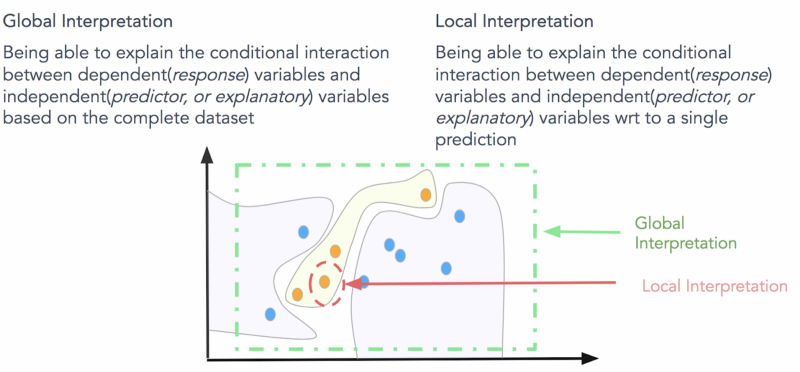
\includegraphics[width=0.9\textwidth]{imgs/global_local.png}
	\caption{Global interpretation view vs. Local interpretation view. Global interpretation explains the feature impact on a global view, based on the whole dataset. Local explanation focuses on the justification for a single instance by inspecting features.}
	\label{fig:global_local}
\end{figure}

\subsubsection{Global interpretation methods}

The global interpretation methods concentrate on the global view of the input variables, more specifically, they identify the most significant features that can largely affect model predictions of the entire dataset. Friedman proposed that the Partial Dependence Plot (PDP) was a global interpretation method which showed the marginal effect of a feature on the model predictions\cite{friedman2001greedy}. This method made clear the relationship between the selected feature and the predictions by adapting the values of the selected feature, and to characterize the feature impact on model predictions. Typically, some simple relationships such as linear or monotonic relation could be inferred from the plot directly. 

Another popular approach is called feature importance. There are many methods for assessment of feature importance. The default feature importance mechanism was proposed and implemented by the inventor of the RandomForest algorithm, which was to add up the Gini decreases for each variable over all trees in the forest and got the average. However, Strobl et al. had demonstrated that this method was biased and was not reliable in scenarios when the selected variable was biased in terms of the scale of measurement\cite{strobl2007bias}. Later, an improved strategy called permutation feature importance was described by Fisher et al. \cite{fisher2018model}. In his approach, the feature importance was estimated by the drop of prediction accuracy of the model after permuting the selected feature. A feature is regarded as "important" if prediction accuracy drops extensively after shuffling feature values as the model depends on the feature for the prediction. Conversely, a feature is "unimportant" if the accuracy is slightly dropped, which means the feature is hardly relied on for the model.

An alternative to permutation feature importance was SHAP feature importance, based on the magnitude of feature contribution using shapley values \cite{molnar2019}. To elucidate the idea, we could assume that the model prediction of an individual instance could be decomposed into feature attributions, and each attribution was estimated by the shapley value. Each feature had a corresponding shapley value for each instance. Thus, over the entire dataset, the SHAP feature importance was indicated by the mean absolute shapley values. 

% Permutation feature importance is based on the decrease in model performance. SHAP is based on magnitude of feature attributions.

\subsubsection{Local Interpretation methods}
%Influences do not provide any explanations about how the variable actually affects the response
Local interpretation methods aim at the instance level explanation which means each instance should be supplied with an explanation identifying the cause to the prediction. Following this idea, it leads us to the local surrogate methods, which are able to explain individual predictions of any black box models faithfully. As a concrete implementation of local surrogate models, Local interpretable model-agnostic explanations (LIME) was initially proposed by Ribeiro et al. \cite{ribeiro2016should}. The general idea was to train an interpretable model to approximate the predictions of the underlying black box model. Since the fitted model was interpretable, we hence could use this explanation model to give detailed explanations.

Another possible approach was to calculate the individual contribution of each feature in an instance to compose the final prediction as described in paper \cite{robnik2008explaining}. Inspired by this idea and the theoretical knowledge from the coalitional game theory, shapley value approach was highlighted to explain instance-level predictions with contributions of each feature values \cite{kononenko2010efficient}. Basically, each feature was assigned an importance score for a particular prediction, and the explanation could be derived from feature importance to some extent. 

However, by exploiting the shapley value approach, it was noticed that only a list of shapley values corresponding to each feature was generated to form an explanation for each model prediction, rather than an explanation model such as LIME, which failed to make judgments about the connections between input changes and prediction changes. To address those problems, Lundberg and Lee \cite{lundberg2017unified} proposed a unified framework for explaining predictions, which was based on the shapley value, and it was named SHAP(SHapley Additive exPlanations). In this unified framework, there was an novel approach called Kernel SHAP, which was the combination of linear LIME and shapley values. In this way, the intuitive connections between these two methods made this approach more promising. Besides, potential techniques to solve the computational performance problem in KernelSHAP was brought up as well. Tree SHAP, one of the variants in SHAP framework, was exhibited to deal with the computational complexity problem particularly for tree-based black box models. It implemented fast and efficient algorithms to calculate shapley values in comparison to Kernel SHAP. In addition, Deep SHAP was designed to improve computational efficiency when deep neural network was applied.


% This approach unified existing explanation methods and brought more clarity to the method space. They introduced the explanation model by treating the explanation of an individual prediction as a model.
\subsection{Review of subgroup discovery technique}

\subsubsection{Definition}
Recent developments of the research filed in knowledge discovery in databases have attracted much attention, where numerous methods are proposed to extract local patterns from large volumes of data  \cite{fayyad1996data}. Apart from the methods for mining local patterns such as discriminative patterns \cite{cheng2008direct} and emerging patterns \cite{dong1999efficient}, subgroup discovery (also called pattern mining) is established as a supervised and descriptive data mining technique. As defined in \cite{herrera2011overview}, in the subgroup discovery task, assuming we have a population of individuals and the corresponding property of interest, it aims to discover subgroups that are statistically "most interesting". To put it another way, the interesting subgroups have the most unusual distributional characteristics with respect to certain property of interest given by the target variable \cite{atzmueller2009fast}.

In a formal definition, the fundamental concepts of subgroup discovery task could be summarized by a quadruple (D, $\Sigma$, T, Q) \cite{lemmerich2014novel}. In the quadruple, D represents the dataset, which is formed by a group of instances. $\Sigma$ means the search space, consisting of a set of selection expressions, and the search space covers all the patterns that are going to be traversed through. Take an example, one of the selectors could look like: "sex=Male AND age>30". T implies the target concepts being exploited in the pattern mining task. Commonly, a single target concept, e.g. binary or numeric, is applied to the mining task. Nevertheless, multi-target concepts are also allowed given the existence of exceptional model mining framework \cite{leman2008exceptional}. Concerning the quality measure criteria, symbolized as Q, it is specified depending on the target concept.

\subsubsection{Quality measure}
To gain more insight, we present some quality measure criteria in this part. Since considerable research efforts have been devoted to study the binary target concept, the quality measure for binary target is well-investigated. One variant of the quality measure for binary target could be easily estimated by the parameters contained in a contingency table, which describes the distribution of positive/negative instances for the observed pattern and its complement subgroup, respectively. According to an investigation by Kloesgen et al. \cite{klosgen1996explora}, they proposed a prevalent family of quality measure, relating to the size of the subgroup and the difference between the target share in the subgroup and the target share in the general population. 

Correspondingly, several approaches to measure the quality of numeric attributes had been proposed, and a list of interestingness measures for numeric target concepts could be found in paper \cite{pieters2010subgroup}. Since a numeric attribute has certain characteristics, such as mean value or median value, therefore, the quality measure for a numeric target could be formalized by slightly adapting the quality function which is designed for binary targets. To be specific, chances were that the share of target in the subgroup and in the entire population could be replaced by the characteristic of the target. Generally, there were five categories of interestingness measure for numeric target, concluded by Lemmerich \cite{lemmerich2014novel}, which were mean-based measures, median-based measures, variance-based measures, distribution-based measures, and rank-based measures. 
Furthermore, as for a multi-target concept, the quality function had been described in a number of studies. And a general framework for multi-target quality functions was the exceptional model mining framework reported by Leman et al. \cite{leman2008exceptional}, proposing a variety of model classes, which contained the correlation model, the regression model, and the classification model class.   

\subsubsection{Subgroup discovery algorithms}
From previous part, four indispensable components were mentioned to define the problem of subgroup discovery. And in the following, algorithms to efficiently execute the subgroup discovery task is going to be considered. 

Unlike the choice of the quality measure which is mainly determined by a target concept in the subgroup discovery task, the mining algorithms are almost equivalent. And for a specific algorithm, three algorithmic components should be verified, which are enumeration strategy, data structure, and pruning strategy. Various enumeration strategies could be used, e.g. exhaustive methods, seeking to acquire the optimal subgroup by traversing through the whole search space. In contrast, heuristic approaches, normally a beam search strategy, was often used for subgroup discovery due to its efficiency, which aimed to find interesting patterns but not necessarily the optimal patterns in a short time \cite{clark1989cn2}. From data structure perspective, data was normally stored in a horizontal layout, e.g. tabular-formatted database. Instead, vertical data representations could also be used, which was covered in paper \cite{zaki2000scalable}. Besides, referring to the wide-spread FP-Growth algorithms, FP-tree structure was also applicable to data \cite{han2000mining}. Furthermore, considering the efficiency of algorithms, the pruning strategies was of critical importance. To determine the upper-quality bounds and safely prune parts of the search space, optimistic estimates could be explored as initially stated by Wrobel et al. \cite{wrobel1997algorithm}. In addition, to shrink the search space of subgroup discovery task, minimal support pruning strategy was useful by exploiting anti-monotone constraints.




\newpage

\section{Approach}
In this chapter, the details of approaches will be discussed. It starts with an overview of local interpretation methods and several variants of them are introduced respectively. Firstly, we present the binary feature flip idea which aims to characterize the impact of binary features by flipping the feature values. After that, we are interested in the effect of numeric features in the model by inspecting the outcome change of the model when the numeric feature values are perturbed to generate noises. Despite the "variable-specific" methods, we also focus on local interpretable model-agnostic explanations (LIME) which is able to explain individual predictions for any types of features and models. However, no theory can support why LIME can fit linear behavior locally on black box models. Therefore, we continue exploring Shapley value, which is a reasonable explanation method with well-founded theory. In addition, the appealing approach assigns a contribution score for each feature value to smooth the path of interpreting the final prediction of individual instances by calculating the Shapley value. 

Then the following section describes the novel technique which combines the local interpretation methods and pattern mining technique. Since the target concept during subgroup discovery in our situation is either prediction change or feature influence score, therefore, the focus shall attribute to numeric target. Later, the standard approaches to measure the interestingness of subgroups are discussed. Furthermore, methods to avoid redundancy in subgroups are explored. 

%TO DO: provide more concrete examples
\section{Local interpretation methods}

In comparison to Global interpretable methods which are dedicated to explain the global model output by comprehending the entire datasets, it is more interesting to examine the model prediction for an individual instance. Besides, it could be observed that the global interpretation methods are less sensitive to noises if we make some perturbations on feature values, however, it could lead to tremendous changes in the prediction for an instance. Therefore, the local explanations shall preserve high accuracy than global explanations. In the following, few local interpretation methods will be covered in detail. 

\subsection{Binary feature value flip}

Binary feature implies that the feature only contains two unique values. In another word, if it is encoded as discrete numeric number, the feature value should be either 1 or 0. Thus, to flip binary feature value means to convert from 1 to 0 or the other way around. In practice, we could also use the XOR operation to map from 1 to 0. For instance, gender is regarded as a binary feature which only holds value "male" and "female". 

As mentioned previously, the assumption is that we hold the dataset and the corresponding model trained on that dataset. Initially, we could obtain the prediction from the model for a specific instance. Then, a binary value is flipped on a chosen feature and afterwards a new prediction is generated by applying the model to the modified instance. Therefore, as a simple measurement, the effect of this binary feature could be estimated by the difference between two outputs. 

In practice, there are two variants to assess the variable influence. One way is to calculate the absolute difference of two predictions, and in this way we could ignore the bias of this binary feature on the original dataset. Literally to say, the binary feature is more influential when the difference becomes larger. In contrast, we could compute the difference for a defined direction, for example, we just care about the effect of gender changing from male to female. In this case, not only the magnitude of the effect is obtained, but also the positive or negative sign towards the prediction.  

\subsection{Numeric feature value perturbation}

As the name suggests, this technique is applicable to features whose type is numeric. The idea is that we could apply binary operations to the input values to produce new values, which serves as injecting noises into the original dataset. In particular, only addition and subtraction are considered in this situation. For example, an instance includes a numeric feature called "age" and we could perturb this feature value by increasing or decreasing by a certain value to obtain the modified value. 

The procedure of measuring the effect of a chosen input feature is similar to that in binary feature value flip approach. For classification or regression tasks, we could make predictions with the existing model on the instance we desire to explain. Afterwards, a new prediction is made on the adapted instance which is produced through perturbation on the selected numeric feature. And the impact of this numeric feature could be approximately evaluated by the absolute difference of two output predictions, which indicates that this particular feature plays an important role in this instance, causing unstable predictions. Roughly to say, larger prediction differences might imply the feature has a stronger effect on the corresponding instance. 


\subsection{Local Surrogate: LIME}

Various criteria can be used to classify types for machine learning interpretability. Intrinsic interpretability, for example, is one type of the interpretability methods, which refers to models that are intrinsic interpretable owing to their simple structures, such as linear models or decision trees. In contrast, post hoc interpretability is meant to analyze the model interpretability after model training. As introduced earlier, permutation feature importance is a post hoc interpretation method. 

In this thesis, we would like to focus on post hoc interpretability, which indicates to explain model decisions after the model has been trained. In particular, model agnostic interpretation methods, which extracts post hoc explanations by treating the original model as a black box, is highly valued. The model agnostic interpretation method is pretty flexible in terms of models, and it can work with any type of machine learning models, which provides a great advantage over model-specific methods \cite{ribeiro2016model}. The principle behind is to learn an interpretable model on the decisions of the black box model and in return apply the interpretable model to those predictions that are expected to explain.  

Following this idea, it leads us to the local surrogate methods, which are able to explain individual predictions of any black box models in a faithful way. As a concrete implementation of local surrogate models, Local interpretable model-agnostic explanations (LIME) was initially proposed in paper \cite{ribeiro2016should}. 
%It might be noticed that the previously presented approaches are constrained within a certain situation and the stability or accuracy is not guaranteed either. Naturally, the aim comes to discover approaches to explain individual predictions of any black box models faithfully, leading us to the local surrogate methods. As a concrete implementation of local surrogate models, Local interpretable model-agnostic explanations (LIME) was initially proposed in paper \cite{ribeiro2016should}. 

The key point behind LIME is pretty straightforward. It is intended to explain individual explanations by fitting a simple interpretable model to locally approximate the underlying black box model. The typical choice of the interpretable model could be regularized linear models like Lasso or decision trees. To elaborate more intuition for LIME, the toy example is shown in \ref{fig:lime}. This is a binary classification task and the regions colored with blue or pink are regarded as two distinct decisions. Evidently, this decision function can not be easily interpreted by a linear model. As a clarification, we are interested in the individual instance explanation, which is marked with a bold red cross. To fit a local interpretable model, some artificial points are created by perturbing the original data point. The learned local model, marked by the dashed line, could in principle provide a faithful explanation for the target instance. 

\begin{figure}[H]% use[!htb] to force the latex ignore the defaut
	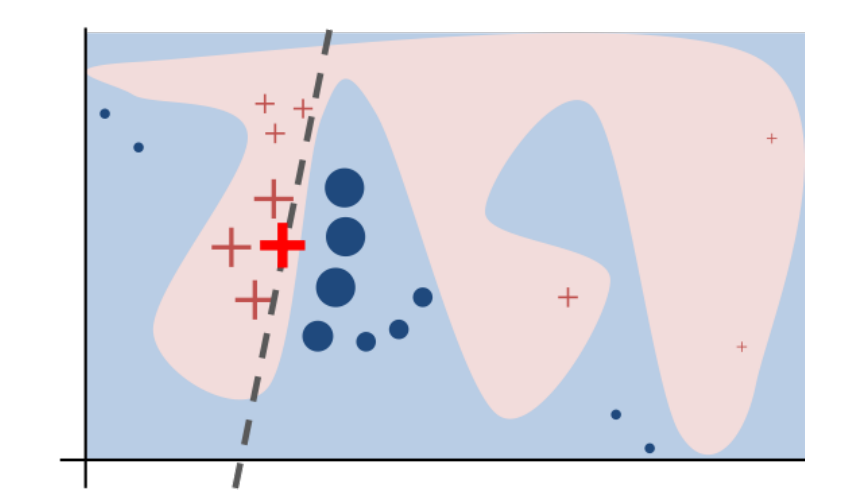
\includegraphics[width=0.9\textwidth]{imgs/lime.png}
	\caption{Binary classification task for a black box model. Decision regions are colored with a blue or pink background. Instance to be explained are marked in a bold red cross. Artificial points, marked as crosses and circles, are created by perturbing the instance of interest, whose size are weighted by the proximity to the instance. The dashed line expresses the fitted local interpretable model which could give faithful explanations.}
	\label{fig:lime}
\end{figure}

Apart from the intuition, we could argue for the faithfulness from a mathematical perspective and the constraint of LIME could be represented as equation \ref{eq:lime}. 

\begin{equation} \label{eq:lime}
\begin{gathered}
\xi=\underset{g \in {G}}{\arg \min } L\left(f, g, \pi_{x}\right)+\Omega(g)
\end{gathered}
\end{equation}

As formally defined in the equation, f is the black box model, g is the local explanation model needs to be figured out, and G is a group of interpretable models, which includes linear models, decision trees, or falling rule lists \cite{wang2015falling}. As depicted in the figure, the weight is measured by the proximity of instance of interest to the surrounding artificial instances, which is defined as $\pi_{x}(z)$. And the complexity of explanation model g is described as $\Omega(g)$. For example, the complexity could be estimated by the depth of trees for decision trees models or by constraining the maximum number of features in linear models. Thus, as seen from the formula, in order to obtain the local explanation model for instance x, the loss L (e.g. mean squared error) should be minimized while maintaining the complexity as low as possible.

In practice, the general procedure to train an explanation model is described as follows: First, select an individual instance that we desire to explain for its black box prediction. Then, generate artificial data points by perturbing the selected sample and make predictions for these new instances using the original model. Afterwards, calculate the weights for new instances according to their proximity to the instance being explained. Next, fit a weighted, interpretable model on the obtained dataset. Finally, interpret the instance prediction by utilizing the trained local interpretable model. 

After a literature review, it is found that LIME is one of the few methods that work for tabular data, text and images, which is a very promising approach. The python implementation is currently available in \cite{lime}, which is still in active development and needs further exploring. 

\subsection{SHapley Additive exPlanations: SHAP}
%In response to this we chose to use a model agnostic representation of feature
%importance, where the impact of each feature on the model is represented using Shapley values

As we have seen, numerous approaches have been recently proposed to explain predictions for individual instances of black box models. As stated in \cite{robnik2008explaining}, the presented approach is relied on the decomposition of a prediction for a single instance on individual contributions of each attribute, and the contribution for each feature value is measured as the difference between the output value and the average output over all perturbations of the corresponding feature. Nevertheless, this approach fails to work if the features are conditionally dependent. 

Inspired by the coalitional game theory which instructs us to fairly distribute the "payout" among the "players", a general method for explaining black box models by taking into account interactions between features can be found in \cite{kononenko2010efficient}, whose fundamental concepts are borrowed to explain instance-level predictions with contributions of each feature values. Corresponding to the known concept in coalitional game theory, the contributions of individual feature values are called Shapley Value.

Despite from the abstract concept, an illustration taken from \cite{molnar2019} might help us intuitively understand the Shapley value. Imagine there is a room and all feature values of an individual instance enter the room in a random order. All feature values, seen as players, need to collaborate with each other to participate the game, where each player contributes to receive the final prediction. And each order of feature values represents a coalition. Consequently, the Shapley value of a feature value corresponds to a difference in the value of a coalition when the feature is added to it. In other words, the Shapley value is the average marginal contribution of a feature value across all possible coalitions. 

Then, let us have a detailed look at the formal definition of Shapley value as expressed in equation \ref{eq:shapley}, where S is the subset of the features in an individual instance, p is the number of features, and x is the vector of feature values of the instance to be interpreted. As for characteristic function val, it describes the contribution of feature j in each coalition.


%The best explanation of a simple model is the model itself; it perfectly represents itself and is easy to understand. For complex models, such as ensemble methods or deep networks, we cannot use the original model as its own best explanation because it is not easy to understand. Instead, we must use a simpler explanation model, which we define as any interpretable approximation of the original model


\begin{equation} \label{eq:shapley}
\phi_{j}(v a l)=\sum_{S \subseteq\left\{x_{1}, \ldots, x_{p}\right\} \backslash\left\{x_{j}\right\}} \frac{|S| !(p-|S|-1) !}{p !}\left(\operatorname{val}\left(S \cup\left\{x_{j}\right\}\right)-\operatorname{val}(S)\right)
\end{equation}

Referred to \cite{shapley1953value}, the Shapley value can provide the unique solution that adheres to he desirable properties, which are Efficiency, Symmetry, Dummy, and Additivity.

\textbf{Efficiency}: denoted as \ref*{eq:efficiency}, which requires that the sum of feature contributions must equal to the difference of the final prediction and the average prediction over all coalitions. 

\begin{equation} \label{eq:efficiency}
\sum_{j=1}^{p} \phi_{j}=\hat{f}(x)-E_{X}(\hat{f}(X))
\end{equation}

\textbf{Symmetry}: The contributions of two feature values j and k are the same, which means equation \ref{eq:symmetry} should be satisfied. 

\begin{equation} \label{eq:symmetry}
\begin{gathered}
\begin{aligned}
if \ val\left(S \cup\left\{x_{j}\right\}\right) &= val\left(S \cup\left\{x_{k}\right\}\right) \\
then \  \phi_{j} &= \phi_{k}
\end{aligned}
\end{gathered}
\end{equation}

\textbf{Dummy}: The contribution of feature j is 0 if it does not change the predictions when it joins into any coalitions. This properties can be demonstrated in equation \ref{eq:dummy}.

\begin{equation} \label{eq:dummy}
\begin{gathered}
\begin{aligned}
if \ val\left(S \cup\left\{x_{j}\right\}\right) &= val\left(S \right) \\
then \  \phi_{j} &= 0
\end{aligned}
\end{gathered}
\end{equation}

\textbf{Additivity}: For any pair of games v, w, the combined payouts should equal to the sum of two individual payouts, as shown in equation \ref{eq:additivity}. For example, if we trained a random forest and the additivity axiom guarantees that we can calculate the Shapley value for each tree respectively then average them to obtain the final Shapley value. 

\begin{equation} \label{eq:additivity}
\begin{gathered}
\begin{aligned}
\phi_{j}(v+w) &= \phi_{j}(v) + \phi_{j}(w) \\
where \ (v+w)(S) &= v(S) + w(S)
\end{aligned}
\end{gathered}
\end{equation}

Though classical Shapley value leads to a potentially promising result, this approach is too computationally expensive owing to computations for the exponential number of possible coalitions. Feasibly, approximation algorithms could be used to reduce the computational complexity, nevertheless, it inevitably will increase the variance for the calculation of Shapley value. What is worse, the explanation for the prediction of a model is just a simple value, rather than an explanation model like LIME, which fails to make judgments about the connections between input change and prediction change. To address those problems, Lundberg and Lee \cite{lundberg2017unified} proposed a unified framework for explaining predictions, which is based on the Shapley value, and they named it SHAP(SHapley Additive exPlanations). This novel approach unifies existing explanation methods and brings more clarity to the methods space. They introduced the explanation model by treating the explanation of an individual prediction as a model. Of course, the unique solution is guaranteed with the game theory. In addition, it provides a more human-understandable and intuitive explanation by user studies as they claimed. 

In this case, SHAP values are introduced as a novel measure of feature contribution. Similar to classical Shapley value estimation methods, SHAP values provide the unique additive feature importance measure if the flowing properties are satisfied, which are Local accuracy, Missingness, and Consistency \cite{lundberg2017unified}. From another perspective, SHAP method transforms the Shapley value approach into an optimization problem by using kernel function to measure proximity of instances. Within this domain, the novel approximation model agnostic method is called kernel SHAP, which is a combination of LIME and Shapley value. In order to use linear explanation model to locally approximate predictions, we should minimize the following objective function \ref{eq:lime}. 

It is intended to obtain the unique solution of equation \ref{eq:lime}, which should also be in line with those three properties, the Shapley kernel is defined as \cite{lundberg2017unified}:

\begin{equation} \label{eq:shap_kernel}
\begin{gathered}
\begin{aligned} \Omega(g) &=0 \\ \pi_{x^{\prime}}\left(z^{\prime}\right) &=\frac{(M-1)}{\left(M \text { choose }\left|z^{\prime}\right|\right)\left|z^{\prime}\right|\left(M-\left|z^{\prime}\right|\right)} \\ L\left(f, g, \pi_{x^{\prime}}\right) &=\sum_{z^{\prime} \in Z}\left[f\left(h_{x}\left(z^{\prime}\right)\right)-g\left(z^{\prime}\right)\right]^{2} \pi_{x^{\prime}}\left(z^{\prime}\right) \end{aligned}
\end{gathered}
\end{equation}
where $|z^\prime|$ is the number of non-zero elements in $z^\prime$

The SHAP framework recently is in active development and is accessible at \cite{shap}. Since it is seemed to be a very optimistic approach and we are quite interested in this novel model explanation method, therefore, further experiments will be conducted. 

\section{Decision trees with Local interpretation methods}
%In the next section, we completely switch gears.

The Decision Tree is a supervised machine learning method used for classification and regression tasks. It is called "Decision tree" because the structure of each decision tree is a tree-like graph and model is constructed to predict the target by learning simple decision rules inferred from data attributes. Decision tree itself is an interpretable model that can provide human-understandable decisions by exploring the decision rules. To be specific, a decision tree applies a recursive partition technique, which keeps on splitting the data based on the selected attributes. From another perspective, it is also a predictive rule-based approach, which could be used to mine local patterns through the decision path, where each path is traversed from the root node to a leaf node. In literature, numerous methods to create decision trees have been proposed and the main difference between decision tree induction strategies is in their attribute selection methods \cite{quinlan1986induction}. 
(Besides, it is worth to be mentioned that the decision tree finds the optimal splitting pattern by essentially limiting the number of conditions to one. \cite{zimmermann2009cluster})


\section{Pattern mining with Local interpretation methods}


Up to now, we have seen a list of local interpretation methods which facilitate us to explain the individual prediction made by the black box model. It is observed that by applying interpretation methods, we obtain an explanation model for each instance regardless of the underlying black box model, meaning that even though the black box model is replaced, the instance-level explanation remains relatively consistent, which is a big advantage in some degree. In principle, it is also assumed that two similar instances would lead to two similar explanation models, which are not supposed to provide two disparate explanations, nevertheless, situations like that could happen in practice. The cause might be attributed to the excessive interpretation of the selected instance, which is merely a sample instance rather than a representative of all instances. Therefore, it comes to our mind that we could discover some potentially useful and valid patterns in instances whose individual explanations are similar, leading us the novel method that combines the subgroup discovery technique with local interpretation methods. 

It could be reminded that pattern mining, whose interchangeable name is subgroup discovery, is a data mining technique which pursues to find subgroups of data instances that present interesting rules with respect to a predefined target variable \cite{herrera2011overview}. And subgroup discovery is a descriptive technique, which tells enough details such that the results are understandable by human experts. Therefore, it is believed that the discovered patterns should provide a more robust explanation for the underlying subgroups which also covers the select instance of interest. In the following part, the details of this novel technique will be elaborated. 

\textbf{Background: subgroup discovery}

Firstly, the theoretical background of subgroup discovery will be introduced as follows. 

Formally, four elements can be considered the most important part when a subgroup discovery technique is applied, whose task is defined by a quadruple (D, $\Sigma$, T, Q). These elements are defined below \cite{atzmueller2004towards} \cite{lemmerich2014novel}: 

\begin{itemize}
	\item D is a dataset and is formed by a set of instances. 
	\item $\Sigma$ constrains the search space, which is made up of subgroup descriptions (patterns). And patterns consist of a set of selection expressions, also known as selectors.
	\item T represents the target variable for this discovery task. Various types of target concept could be identified, including binary, numeric or complex. 
	\item Q defines the quality measure criteria. Different quality measures are specified for different types of target. 
\end{itemize}

Using a binary variable as the target of subgroup discovery is a more simple and general situation. Since the binary variable only contains two values (True or False), it is aimed to identify interesting subgroups for each of the possible value. Basically, the idea is to discover patterns whose target share is either remarkably high or remarkably low. However, pattern mining for numeric target is more complicated because the variable can be dealt with in a numerous ways such as numeric target discretization in a predefined number of intervals, or dividing the numeric domain into two ranges with respect to the average. 

Recall from local interpretation methods, the contribution values for each variable of an individual instance could be obtained by using the explanation model to interpret the black box model. In this case, the contribution score of the chosen variable is our target, which is naturally to be numeric. Now, the next step goes to the traditional pattern mining problem, aiming to discover subgroups of the population that are statistically interesting. 

\textbf{Interestingness measure for numeric target}

Unlike binary target situation where interestingness measures are easy to investigate and research, the quality measure for numeric target becomes more complex. Nevertheless, a list of interestingness measure for numeric target could be found in \cite{klosgen2002data}. And a substantial discussion about quality measure could also be traced in \cite{pieters2010subgroup}. As could be summarized, a numeric attribute has a certain number of characteristics, such as the mean value or the median value. From that perspective, it could be imagined to specify interestingness measure for the numeric target with respect to those predefined data statistics. In this case, by comparing the statistics in the subgroups and in the entire population, the interesting groups will be discovered. Generally, there are five categories of interestingness measure for numeric target, concluded in \cite{lemmerich2014novel}, which are mean-based measures, median-based measures, variance-based measures, distribution-based measures, and rank-based measures. Among all of them, the details of mean-based measures will be extended since they are adopted in the experimental phase. 

To elaborate a bit more, measuring the quality of a specific subgroup depends on the difference between the mean value in the subgroup and the mean value in the entire dataset. The general formulation is denoted in equation \ref{eq:mean_based}, where $i_{P}$ is the size of the subgroup, $a$ is a parameter which weights the subgroup size and deviations, and $\mu_{P}, \mu_{\emptyset}$ represent the mean value in the subgroup and the mean value in the dataset respectively. In particular, the choice of parameter $a$ could be selected in an iterative process. For example, $a$ is incremented if the subgroup size is too small to have a significant score, meanwhile, low parameter values for $a$ is preferred with a high deviation of mean target values between the subgroup and the overall dataset. Therefore, after calculating the quality score for each subgroup, those subgroups with significantly higher or lower mean values are considered as interesting and the descriptions of them are our desirable interesting patterns. 

\begin{equation}  \label{eq:mean_based}
q_{m e a n}^{a}(P)=i_{P}^{a} \cdot\left(\mu_{P}-\mu_{\emptyset}\right), a \in[0,1]
\end{equation}

\textbf{Redundancy Avoidance}

Though patterns could be discovered through the traditional interestingness measure presented above, the results are not ideal, which contains too many redundant patterns. In the quality measure, only the subgroup size and statistics difference between subgroups and entire dataset are considered, which might produce uninteresting patterns when ignoring the selector expressions of subgroups. For example, assume that the mean contributions of age for the entire dataset is at $M_{\emptyset}=0.50$. And the mean value in the subgroup with the expression $age > 40 \cup gender=male$ is $M_{age > 40 \cup gender=male}=0.80$. It seems that the pattern should have a high quality score and is identified as an interesting pattern. However, it is probably not interesting enough if given the information that its generalization has nearly the same value, which means mean value does not deviate significantly from the mean value of its generalizations, e.g. $M_{age > 40} = 0.78$. 

To avoid that such subgroups are included in the result set, Generalization-aware interestingness measures could be applied to improve the traditional selection criteria for pattern mining by considering the statistics of the subgroup and also to its all generalizations. In \cite{grosskreutz2010subgroup}, Grosskreutz et al proposed to estimate the quality of a pattern $P$ as the minimum of the quality of $P$ with respect to the extension of all its generalizations. Denoted as equation \ref{eq:incremental_q}, $q^{\Delta}$ is the incremental version of q, $D$ is the dataset, $P$ is the subgroup and $H$ includes its all generalizations. 

\begin{equation} \label{eq:incremental_q}
q^{\Delta}(D B, P)=\min _{H \subset P} q\left(D B\left[H\right], P\right)
\end{equation}

Since the mean value of the target is mainly explored, the above equation could be formalized in a simpler way, as shown in \ref{eq:generalization_q}. By doing so, redundant patterns are avoided and more interesting subgroups are discovered. 

\begin{equation} \label{eq:generalization_q}
q_{\operatorname{mean}}^{a}(P)=i_{P}^{a} \cdot\left(\mu_{P}-\max _{H \subset P} \mu_{H}\right), a \in[0,1]
\end{equation}

\textbf{Search strategy}
Apart from the quality measure, the search strategy is critical since the dimension of the search space and time complexity if of great concern. Various strategies could be used, e.g. exhaustive methods, seeking to acquire the optimal subgroup by traversing through the whole search space. In contrast, heuristic approaches, normally a beam search strategy \cite{clark1989cn2}, is often used for subgroup discovery due to its efficiency, which aims to find interesting patterns but not necessarily the optimal patterns in a short time. The intuition behind is that it is assumed that the patterns are more likely to be interesting if their generalizations are also interesting. Therefore, the search starts with an empty hypothesis, then it tries to find the best patterns with size k (corresponding to beam width) by evaluating all selectors in the subgroup discovery task. Following that, at each search iteration, the hypotheses contained in the beam are expanded but only the currently best w hypotheses are kept using a hill-climbing greedy search \cite{atzmueller2015subgroup}. 





\newpage

\section{Experiments}
After a detailed introduction to methodology , in this chapter, we will concentrate on practical experiments. To begin with, datasets that will be utilized in the experiments will be introduced, including the well-known UCI datasets and the artificial dataset. Next, a general overview of the classification or regression models that might be encountered in the experiments is provided. Then, we intend to compare different local interpretation methods on the same dataset and give explanations on the feature that is interested. To interpret the feature explanation for an individual instance and discover the interesting patterns, subgroup discovery technique is applied. As a comparison, decision tree visualization is exposed to find local patterns. And finally, we will apply the promising SHAP approach to conduct case studies on real datasets. 

\section{Datasets}


\subsection{Artificial dataset}

Before exploring the local interpretation methods on real datasets, we would like to justify the concept that interesting subgroups could be recovered from the artificial dataset by inspecting variable influence. Presumably, there were hidden patterns in the synthetic dataset that were useful to provide reasonable explanation to the predictions. By interpreting the effect of a certain variable, e.g. gender, it was assumed that the interesting pattern could be recovered. The procedure to construct an artificial dataset and conduct experiments will be described as follows. 

For simplicity, we constructed the artificial dataset relying on the popular "Adult Income" dataset, but we only extracted partial information, which meant that only the information about age, education-num, sex, hours-per-week and income were included. As assumed, the synthetic data contained some interesting patterns, such as "age < 30". One exemplary case was that when "age < 30", the attribute "gender" had stronger effect on predictions while in its complementary subgroup, the effect of "gender" was slight. And the task was indeed to discover this pattern by exploring the effect of gender. 

For further experiments, one way to fabricate this interesting pattern was to modify the gender effect directly on the corresponding subgroups. For instance, if the condition that "age < 30" was met, we could manually add 3 unit in terms of the scale of measurement on gender effect, and otherwise we could subtract 3 unit. Another idea was to establish two models that behaved differently when considering this condition. It is known that the coefficients in the logistic regression model have straightforward interpretation, indicating the influence level by the input features. Therefore, we could create two distinct models by changing the weights of the features in accordance with the previous defined patterns, which was that when "age < 30", the effect of gender was relative large. In specific, we could assign larger weights to the model that was applied on the pre-described subgroup to maintain larger gender effect, while decreasing feature weights on the model that was applied on its complementary subgroup.

In this paper, we would like to adopt the latter method to make up the synthetic dataset and build the models. 

\subsection{UCI datasets}

Apart from the synthetic dataset, we will mostly consider datasets that could be found in UCI Machine Learning Repository \cite{asuncion2007uci}. Ideally, we would like to choose datasets that covers various domains, including social, financial and life science areas. Therefore, for classification tasks, concerning the popularity and quality of datasets, we decided to adopt the "Adult Income", "German Credit", and "Breast Cancer Wisconsin" datasets. In Adult Income dataset, there are 14 descriptive features and more than 40 thousand instances, which were extracted from US census database. And the task was to predict whether a person earned more than 50K a year or not. As for the German Credit dataset, it was determined to figure out whether a person had good or bad credit risks relying on the 20 descriptive attributes for each person. It is worth mentioning that these two datasets contain multivariate data types, consisting of categorical features and numerical features. In that regard, data preprocessing needs to be considered in addition. Another Breast Cancer dataset is composed of 32 features and all of them are numerical features except for the predicted label which tells whether the diagnosis of cancer is malignant or benign. Those features of an individual instance are extracted from an image of a breast mass, which describes the characteristics of the cell nuclei in the image. 

For regression tasks, we specifically choose the "Bike Sharing" and "Boston Housing" datasets. In Bike sharing dataset, the task is to predict the count of total rental bikes within a specific time frame. It is made up with 17389 entries and each with 16 distinct features. Regarding the Boston housing dataset, it is derived from US census service concerning housing price in the area of Boston MA. 505 records can be found in the dataset and each record contains 14 numerical features. 

In summary, a general overview of real-world datasets that will be used in experiments is concluded in Table \ref{datasets}

\begin{table}[H] \label{datasets}
	\centering 
	\caption{Datasets used in experiments}
	\ra{1.3}
	\begin{tabular}{{m}{3cm}cccc}\toprule[0.5mm]
		Datasets & Usage & \#Instances & \#Features \\ 
		\midrule[0.3mm]
		Adult Income & Classification & 48842 & 14 \\
		German Credit & Classification & 1000 & 20 \\
		Breast Cancer & Classification & 569 & 32 \\
		Bike Sharing & Regression & 17389 & 16 \\
		Boston Housing & regression & 505 & 14 \\
		\bottomrule[0.5mm]
	\end{tabular}
	
\end{table}


%\subsection{Datasets description}
%
%\subsubsection{Artificial dataset}
%
%\subsubsection{UCI datasets}



%\subsection{Data preprocessing }


\section{Experiments setup}


\subsection{Machine learning models}

The first machine learning algorithm that will be used in experiments is Random Forest, which is an ensemble method for classification or regression tasks by creating multiple decision trees at training time. 

Another black box model is gradient boosting trees, which constructs an ensemble of decision trees to perform classification or regression tasks, where each decision tree is a weak prediction model. 
The gradient boosting trees algorithm requires definition of loss function that can be minimized. The algorithm is called boosting because it builds decision trees iteratively. It creates the first tree and finds the data points with high prediction errors, this errors show which data points should be emphasized by the next decision tree. After building all the decision trees, their predictions of these trees are combined by weighted average, where weight depends on a performance of a tree. Different approaches of building gradient boosting trees depend on many hyperparameters and is an active area of research [112]

%The library that is used for gradient boosting trees in this thesis is called XGBoost [111]. The gradient boosting trees algorithm implemented in XGBoost were a part of winning solutions of multiple machine learning competitions [113], including competitions in natural language processing field. The library also works natively with scipy sparse data format and can convert it to an internal data format, called DMatrix, which speeds up the training process. The main parameters of the algo- rithm are max_depth, num_boost_round and learning_rate. The maximal number of splits that allowed in a tree is defined by max_depth, and the number of trees in an ensemble is determined by num_boost_round. The learning_rate parameter enables regularization of the model, by forcing the algorithm to build more trees to achieve the same score. The XGBoost library also allows the usage of validation set, to stop training if the score on validation data did not improve for a given amount of boosting rounds.

deep neural network

%Another machine learning algorithm that will be used with produced feature vectors is gradient boosting trees [110]. The algorithm creates an ensemble of decision trees that perform classification or regression, where each tree is a weak prediction model. A decision tree is a tree-like graph, where each node represents the split based on one of the features in a feature vector. Figure 12 shows an example with two trees, the nodes represent the ‘decisions’ that split the data into subgroups. In case of ensemble models, the trees are called weak because they are intentionally limited by depth [110].
%The gradient boosting trees algorithm requires definition of loss function that can be minimized. The algorithm is called boosting because it builds decision trees iteratively. It creates the first tree and finds the data points with high prediction errors, this errors show which data points should be emphasized by the next decision tree. After building all the decision trees, their predictions of these trees are combined by weighted average, where weight depends on a performance of a tree. Different approaches of building gradient boosting trees depend on many hyperparameters and is an active area of research [112]. More detailed description of this approach is beyond the scope of this thesis.
%The library that is used for gradient boosting trees in this thesis is called XGBoost [111]. The gradient boosting trees algorithm implemented in XGBoost were a part of winning solutions of multiple machine learning competitions [113], including competitions in natural language processing field. The library also works natively with scipy sparse data format and can convert it to an internal data format, called DMatrix, which speeds up the training process. The main parameters of the algo- rithm are max_depth, num_boost_round and learning_rate. The maximal number of splits that allowed in a tree is defined by max_depth, and the number of trees in an ensemble is determined by num_boost_round. The learning_rate parameter enables regularization of the model, by forcing the algorithm to build more trees to achieve the same score. The XGBoost library also allows the usage of validation set, to stop training if the score on validation data did not improve for a given amount of boosting rounds.
%The gradient boosting trees algorithm is a non-linear algorithm, which means that it can approximate more complex data, but without proper regularization can easily overfit. The non-linear nature of the algorithm means signifies that there is no linear dependency between features (i.e., words) and the target class. But because during the construction of decision trees only the most significant features are used, it is possible to sort features by their importance to a given task. Therefore, in our task, we will be able to use this functionality to extract words that had the most influence in predicting the gender based on the text of the comment.

\subsection{Recover patterns on artificial dataset} 

%Before exploring the local interpretation methods, we would like to justify the concept that interesting subgroups could be recovered from the artificial dataset by inspecting variable influence. Presumably, there were hidden patterns in the synthetic dataset that were useful to provide reasonable explanation to the predictions. By interpreting the effect of a certain variable, e.g. gender, it was assumed that the interesting pattern could be recovered. The procedure to construct an artificial dataset and conduct experiments will be described as follows. 
%
%For simplicity, we constructed the artificial dataset relying on the popular adult dataset, but we only extracted partial information, which meant that only the information about age, education-num, sex, hours-per-week and income were included. As assumed, the synthetic data contained some interesting patterns, such as "age < 30". One exemplary case was that when "age < 30", the attribute "gender" had stronger effect on predictions while in its complementary subgroup, the effect of "gender" was slight. And the task was indeed to discover this pattern by exploring the effect of gender. For further experiments, one way to fabricate the interesting pattern was to modify the gender effect directly on the corresponding subgroups. For instance, if the condition that "age < 30" was met, we could manually add 3 unit in terms of the scale of measurement on gender effect, and otherwise we could subtract 3 unit. Another idea was to establish two models that behaved differently when considering this condition. It is known that the coefficients in the logistic regression model have straightforward interpretation, indicating the influence level by the input features. Therefore, we could create two distinct models by changing the weights of the features in accordance with the previous defined patterns. In specific, we could assign larger weights to the model that was applied on the pre-described subgroup to maintain larger gender effect, while decreasing feature weights on the model that was applied on its complementary subgroup.

As clarified earlier, the artificial dataset was constructed based on Adult dataset with a hidden pattern indicating that the gender had large impact on the prediction when "age < 30". Therefore, the aim was trying to verify whether this interesting subgroup could be recovered by pattern mining technique. 

Firstly, to measure the gender effect, we could simply use the binary flip approach described in previous chapter. By flipping the gender value, i.e. transform from "male" to "female" or the other way around, the prediction change denoted as probability was calculated and roughly it was regarded as the effect of gender. Then, treating the effect of gender as the target concept, subgroup discovery technique was applied on the artificial dataset to discover interesting subgroups. It could be observed that these interesting subgroups include the subgroup that were artificially generated in the dataset. The detailed results were left to the next chapter. In conclusion, it could be proved that subgroup discovery technique could indeed provide us patterns of explanations that facilitate us to understand the predictions. 





\subsection{Comparison of different local interpretation methods}

datasets: adult, credit-g, housing
binary flip: perturbation, LIME, SHAP

numeric perturbation: perturbation, LIME, SHAP

classification vs. regression

decision tree vs. subgroup discovery

\subsection{Case Study}

real world case study 2-3 datasets
\newpage

\section{Results and Discussion}
Results...

\subsection{Experiment Results}


% \subsection{Synthetic model evaluation}

\subsubsection{Local interpretation methods comparison}
As was pointed out before, in this experiment, the Breast Cancer dataset was examined. After exploring the dataset, it was noticed that the attribute “area\_mean” was one of the most important features according to the permutation feature importance ranking. Without loss of generality, we could randomly choose one instance and try to provide reasonable explanations. In this scenario, we decided to choose instance 10 from the dataset, and the boosting algorithm was utilized to train a black box model. Therefore, the following results were demonstrated based on the experiment that was intended to inspect the variable “area\_mean” in an ensemble model on the processed dataset. 

First local interpretation approach was numeric perturbation, which was applicable only to numeric attribute. The assumption was that we already had the black box model and the selected instance being explained. It could be easily estimated that there was 89% chance to be predicted as a malignant cancer. Nonetheless, if we deviated the “are_mean” value of the instance by one positive and negative standard value, the probability would increase 0.5% and decrease 65% respectively. In a sense, we could argue that this attribute played a critical role when making predictions. 

The next local interpretation method was LIME. After selecting the instance of interest, it was required to generate neighborhood points by perturbing the instance. To be more specific, the neighborhood points were produced by sampling from Normal(0, 1), multiplying by the standard deviation and adding back the mean value. Then, a weighted intrinsic interpretable model was fitted to explain the prediction making by the classifier. In this way, the model was supposed to be locally faithful around the explained instance. As displayed in Fig~\ref{fig:breast_lime}, the classifier determined that the cancer was malignant with probability 0.89. It could be noticed that features, such as “area\_mean” or “texture\_mean”, had huge impact on the prediction due to the large coefficient in the model. Note that this approach would discretize numerical feature values into quartiles. For instance, it was observed that when the condition “area\_mean > 0.27” was met, the weight for this feature was 0.35. It could be interpreted that if we decreased one unit on this feature value, the chance of the cancer to be malignant would decline 0.35. And on the right side, the feature value pairs of the instance to be explained was displayed in a table format. The feature columns showed the feature names and the value column displayed the original value for the corresponding feature. 

\begin{figure}[H]
	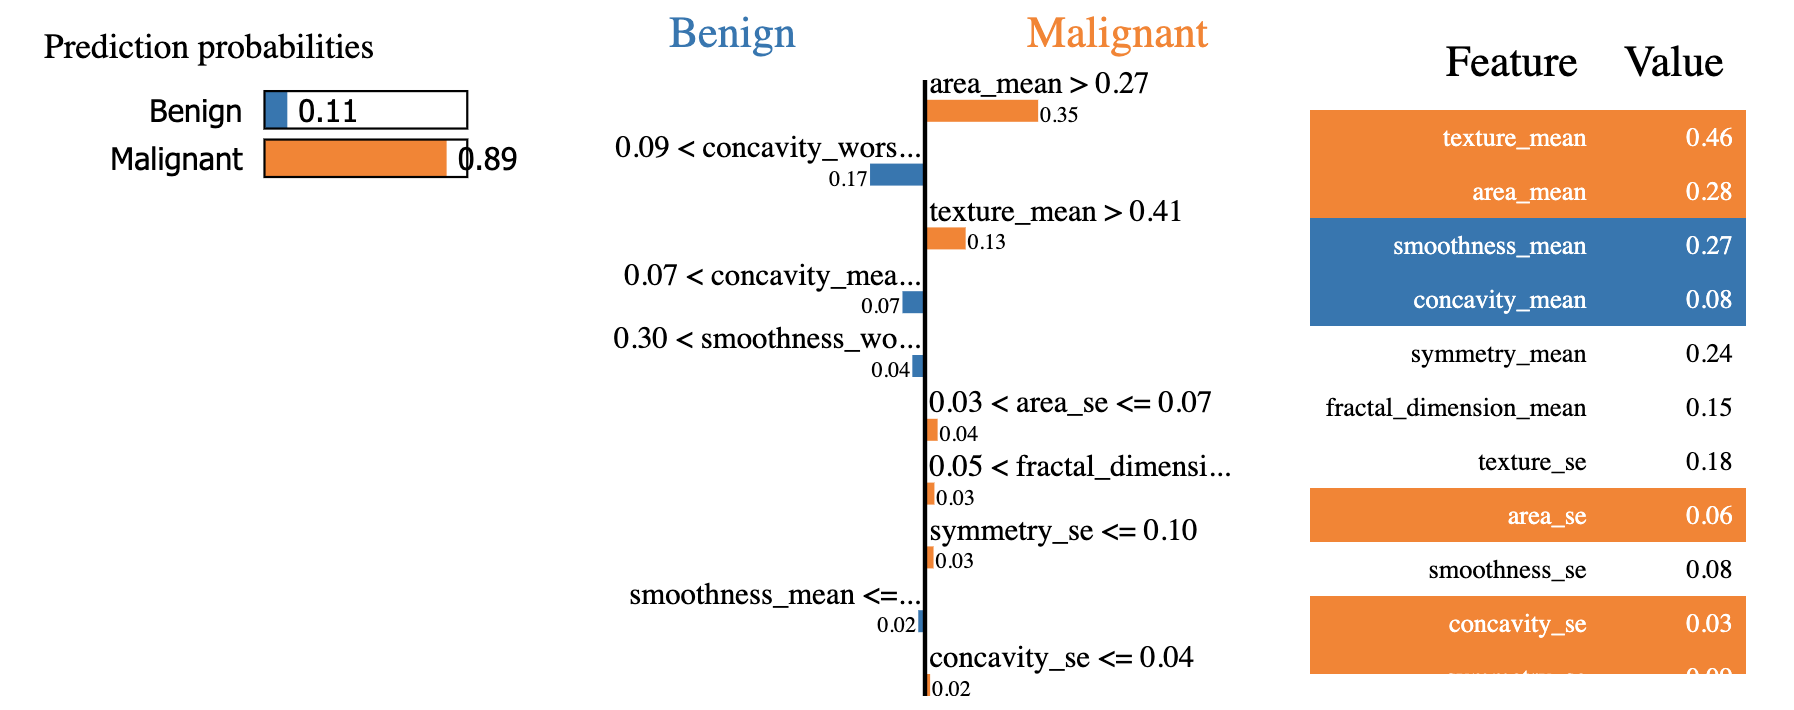
\includegraphics[width=0.9\textwidth]{imgs/breast_lime_plot.png}
	\caption{On the left side, the prediction probabilities were shown, telling that the tumor had 89\% chance to be predicted as malignant. In the middle, the feature weights in the fitted model were  displayed. In particular, the weight for attribute “area\_mean” is 0.35. Note that the feature value pair of the instance being explained were listed on the right side.}
	\label{fig:breast_lime}
\end{figure}

Another local explanation method that we adopted was Kernel SHAP. Nonetheless, despite the fact that the back box model here we trained was tree ensemble model, the more efficient TreeSHAP estimation could be used instead. By applying this approach, it was aimed to compute shapley values for each feature, which were regarded as the feature contributions. As depicted in Fig~\ref{fig:breast_shap} , it gave a nice reasoning which showed feature influence on this prediction. The shapley value could be visualized as “forces” and each feature value was a force either increased or decreased the prediction. As was seen, there was a base value denoted as -1.44, which was the average model output over all predictions. The below explanation showed features each contributing to push the model output from the base value to the actual model output. Features pushing the prediction higher were shown in red, those pushing the prediction lower were in blue. The shapley value for each feature was attached in the figure, but it had to be noted that by default the shapley value were displayed in the logit space and all those shapley values summed up to the difference between the model output for that instance and the expected base value. Therefore, we could infer that for this instance, attributes “area\_mean” and “area\_se” had a dominant effect on the prediction, while “concavity\_worst” had reverse impact. 

\begin{figure}[H]
	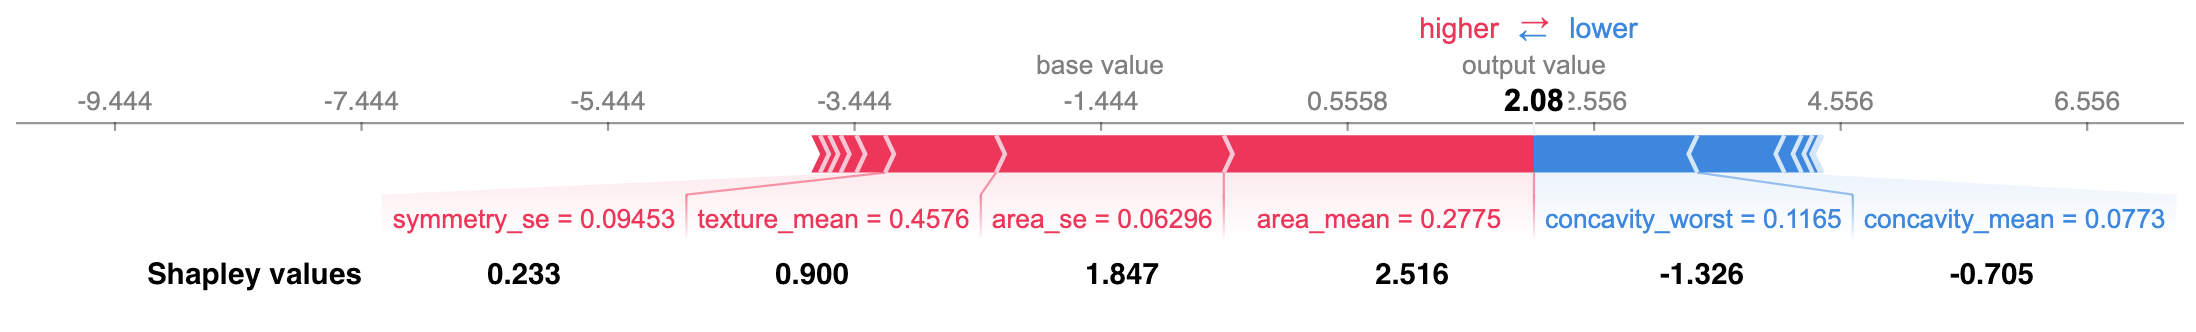
\includegraphics[width=0.9\textwidth]{imgs/breast_shap_force_plot.png}
	\caption{SHAP values to explain the influence of features leading to the prediction of benign or malignant cancer. The base value was the average probability over all predictions in logit space, which was -1.44. Shapley values were attached for each feature value as well. Feature values shown in red had positive effect in increasing the risk of being malignant cancer, while feature values denoted in blue declined the probability.}
	\label{fig:breast_shap}
\end{figure}

\subsubsection{Decision tree vs. Subgroup discovery}

Given the fact that both decision tree algorithm and subgroup discovery technique could be used to discover hidden pattern in data with respect to the effect of a specific attribute, it could be interesting to have a comparison. In this experiment, we decided to choose German Credit dataset, with the aim to predict whether a person has a good or bad credit risk. Since this dataset contained multivariate attributes, the dataset was processed by dummy encoding in this scenario. After exploring the dataset, the attribute “Credit amount” was selected to inspect the effect in the dataset. Thus, the first step was to measure the impact of feature “Credit amount” in each individual instance. In principle, all those aforementioned local interpretation methods supported the feature effect measurement. Nevertheless, Kernel SHAP approach was finally chosen. Following this approach, the shapley value of attribute “Credit amount” was computed for each instance. 

By taking the shapley values as the target, it was assumed that local patterns could describe the influence of the selected attribute in the dataset. In this case, a tree-like graph could be drawn based on the decision tree algorithm. It had to be noticed that the maximal tree depth was set to three. As demonstrated in Fig~\ref{fig:credit_decision_tree}, the first splitting node was “Purpose=furniture/equipment”. By following the rightmost path, it led us to a pattern with high value, meaning that the attribute “Credit amount” revealed a significant impact on the dataset complied with this pattern. This pattern could be described as “Purpose=furniture/equipment AND Duration >13.5 AND Age > 31.5”. 

\begin{figure}[H]
	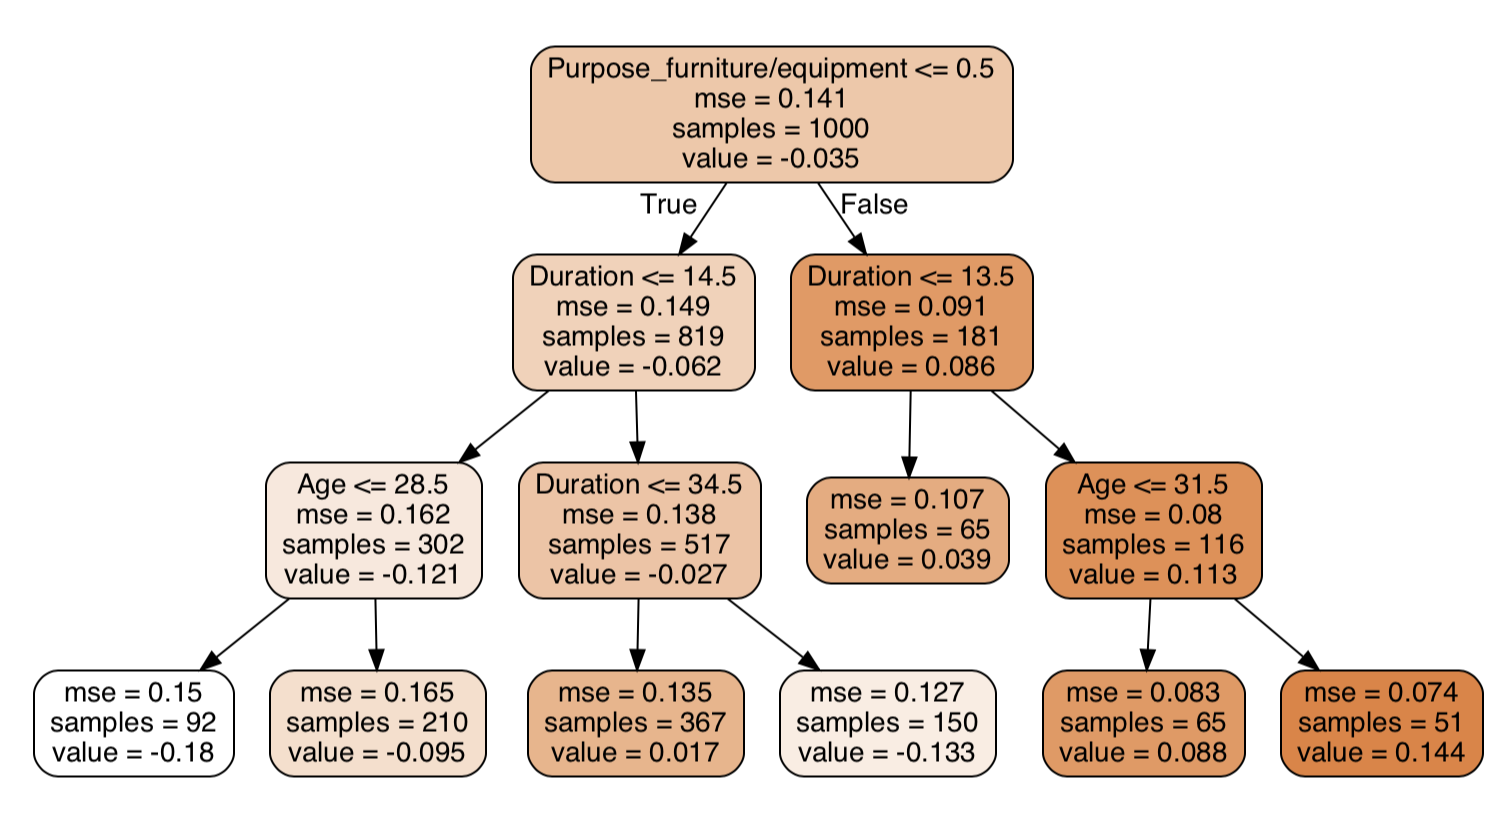
\includegraphics[width=0.9\textwidth]{imgs/credit_decision_tree.png}
	\caption{Decision tree}
	\label{fig:credit_decision_tree}
\end{figure}

In contrast, by considering the shapley value as the numeric target in subgroup discovery technique, those interesting subgroups could be found out as shown in Table~\ref{fig:credit_subgroup}. As could be seen, the average shapley value over the entire dataset was about -0.03, while this value was 0.08 in the subgroup “Purpose=furniture/equipment”, which also corresponded to the first splitting node. And the patterns “Duration >13.5” and “Age > 31.5” depicted in the path along the decision tree was also covered by the discovered subgroups in the table. 

\begin{figure}[H]
	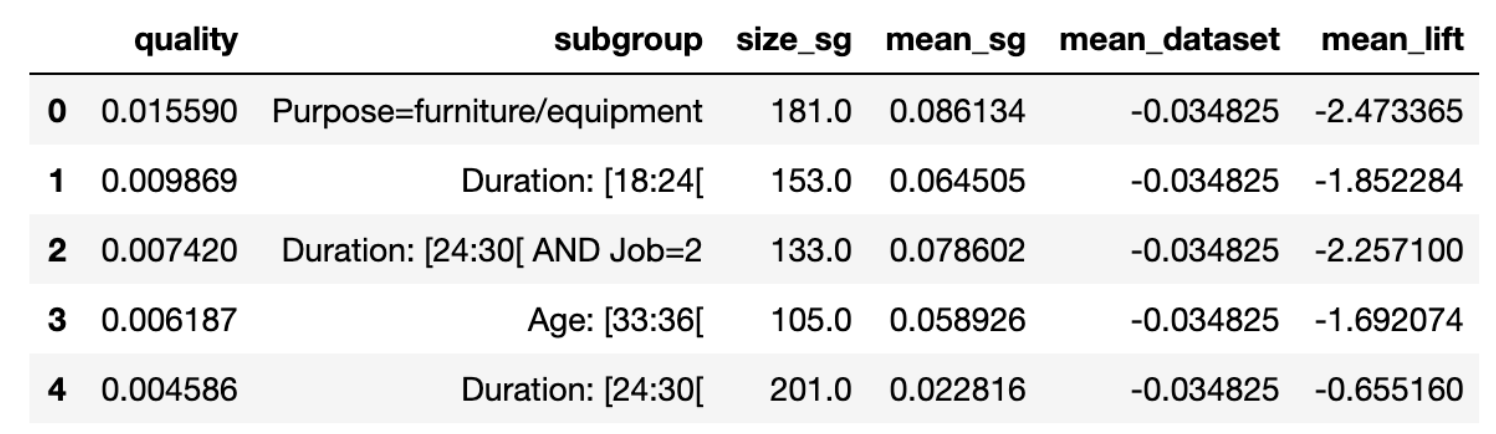
\includegraphics[width=0.9\textwidth]{imgs/credit_subgroup.png}
	\caption{Subgroup discovery results}
	\label{fig:credit_subgroup}
\end{figure}

Considering the similar patterns discovered by both techniques, we might argue that there indeed existed some patterns that the feature had a significant impact, and further influenced the model prediction.

\subsubsection{Case study} 
As clarified in the last chapter, the first case study was experimented on the Adult Income dataset. The task for the experiment was to interpret the influence of a specific attribute in a black box model, and we assumed that the dataset and the model was provided. Initially, the dataset was processed as before by encoding the data and removing correlated features. Afterwards we randomly split the dataset into training set and testing set, and a simple full-connected neural network was trained based on the training data. By far, we had the neural network model and testing data, and the next step was to find out impact of a particular feature in a single instance. Furthermore, we were asked to discover some subgroups where the inspected feature had a dominant influence. 

At the beginning, the importance of each feature was explored, which gave an indication about features that were worthy of attention. Apart from the permutation feature importance approach to estimate the importance degree of each feature, an alternative method to measure the importance was based on the magnitude of feature contributions using shapley values, called SHAP feature importance measure. The intuition was that features with large mean absolute shapley values were important. From the Fig~\ref{fig:adult_bar}, we could tell that “age” was the most important feature comparative to others. Considering that we would like to further compare the pattern mining results based on the feature effects calculated by binary flip approach and kernel SHAP approach, the attribute “sex” was chosen to explore since the binary flip method was designed for exploiting the  binary feature. 

\begin{figure}[H]
	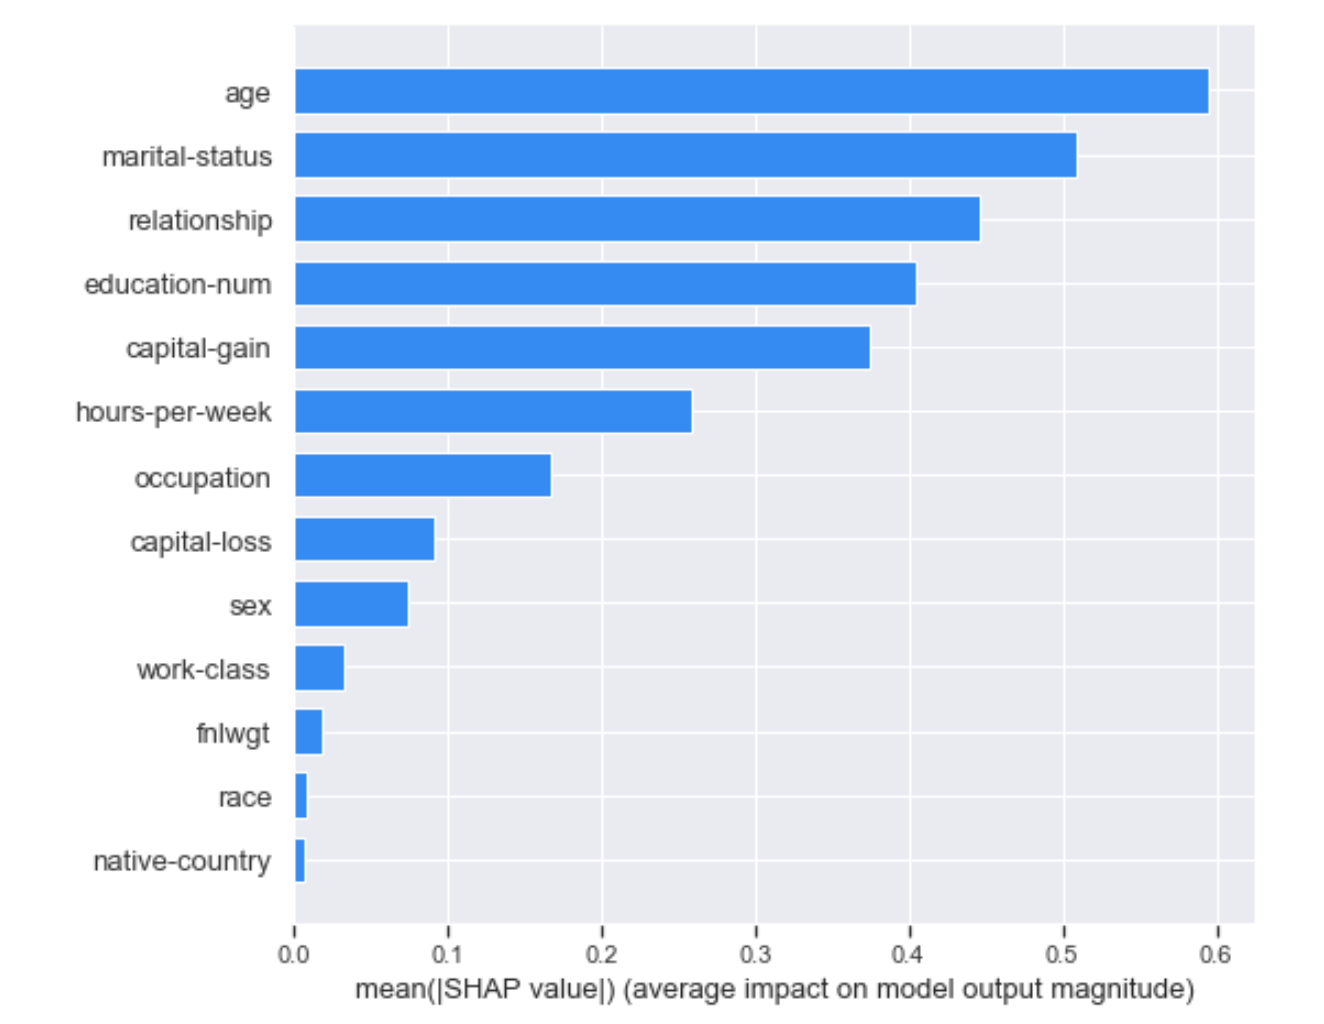
\includegraphics[width=0.9\textwidth]{imgs/adult_bar_plot.png}
	\caption{SHAP feature importance measure was based on the magnitude of feature contributions, and it was assessed by the mean absolute shapley values. “Age” was the most important feature.}
	\label{fig:adult_bar}
\end{figure}

From binary flip method, we could obtain the effect when changing the sex for each instance by calculating the prediction change. As for the kernel SHAP approach, the effect of sex was estimated by this feature contribution by computing the shapley values. Then subgroup discovery technique was applied to the dataset while taking the effect of sex as the target. Therefore, two different results were combined with respect to two different measurements and they were displayed in Table~\ref{fig:adult_subgroup}. Each part represented the interesting subgroups that were discovered. From Table~\ref{fig:adult_subgroup}, it was noticed that these two results were similar in some degree. For instance, they both discovered the pattern such as “relationship=Husband” and “marital-status=Married-civ-spouse”. 

\begin{figure}[H]
	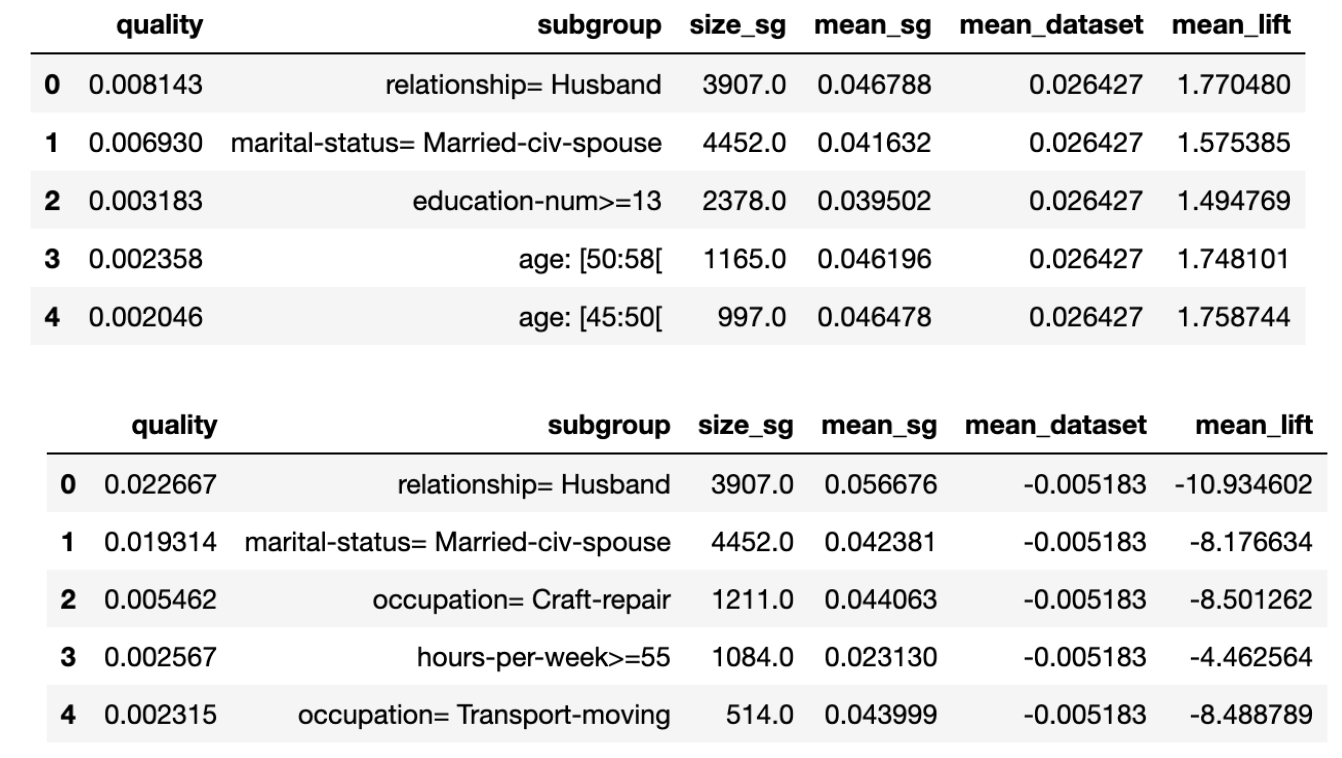
\includegraphics[width=0.9\textwidth]{imgs/adult_subgroup.png}
	\caption{Subgroup discovery results}
	\label{fig:adult_subgroup}
\end{figure}

It could be concluded that there were patterns in data that feature “sex” had a huge impact no matter what local interpretation methods were used. 

\newpage

\section{Conclusion and Future work}
conclusion and future work...

\section{Conclusion and Feature work}


\subsection{Factors to consider}
Conclusion: Local surrogate models, with LIME as a concrete implementation, are very promising. But the method is still in development phase and many problems need to be solved before it can be safely applied.
\subsection{Summary}

\subsection{Outlook}
\newpage

\bibliographystyle{IEEEtran}
\bibliography{reference}
%\begin{thebibliography}{99}
% NOTE: change the "9" above to "99" if you have MORE THAN 10 references.
% chapter 1 
\bibitem{sn} S. Nakamoto, \textit{Bitcoin: A peer-to-peer electronic cash system,} 2008.

\bibitem{c-1} Kasey Panetta \textit{Gartner’s Top 10 Strategic Technology Trends for 2017(2018)} Gartner, Inc., 2007(2018).   

\bibitem{c-Deloi} Sarah Underwood, \textit{Blockchain beyond Bitcoin,} Communications of the ACM, Vol. 59, No. 11. (November 2016), pp. 15-17, doi:10.1145/2994581

% chapter 2
\bibitem{DoubleSpend} Chohan, Usman W., The Double Spending Problem and Cryptocurrencies (December 19, 2017).

\bibitem{pbft} Hamida, Elyes Ben, et al. \textit{Blockchain for enterprise: overview, opportunities and challenges.} The Thirteenth International Conference on Wireless and Mobile Communications (ICWMC 2017). 2017.

\bibitem{tendermint} J. Kwon, \textit{Tendermint: Consensus without mining}, URL http://tendermint. com/docs/tendermint { } v04. pdf, 2014.
 
\bibitem{WBank} H. Natarajan, S. K. Krause, and H. L. Gradstein, \textit{Distributed Ledger Technology (DLT) and blockchain,} The World Bank, Tech. Rep. 122140, Dec. 2017. [Online].
Available: http://documents.worldbank.org/curated/en/177911513714062215/Distributed-
Ledger-Technology-DLT-and-blockchain

\bibitem{sawtooth} https://sawtooth.hyperledger.org/docs/core/releases/latest/introduction.html

\bibitem{dao} https://blockchainhub.net/dao-decentralized-autonomous-organization/

\bibitem{EthereumWhitePaper} Ethereum community \textit{Ethereum Homestead Documentation-Release 0.1}

\bibitem{JapanS}Survey on Blockchain Technologies and Related Services,2016,Nomura Research Institute.
% Chapter 3{\tiny }
\bibitem{sc1} For SCM related to services, see for example the Association of Employment and Learning Providers' Supply Chain Management Guide at aelp.org.uk published 2013, accessed 31 March 2015

\bibitem{sc2} Simon Ellis and John Santagate \textit{The Digitally Enabled Supply Chain with Manufacturing Use Cases},IDC-US42434217

\bibitem{lufthansa} https://www.lufthansa-industry-solutions.com/de-de/loesungen-produkte/supply-chain-logistik-40/innovative-logistik-dienstleistungen-aus-der-box/

\bibitem{sc3} IDC Manufacturing Insights \textit{The Path to a Thinking Supply Chain}

\bibitem{stateA} P.Schiegg,R.Roesgen, H.Mittermayer,
and V.Stich  \textit{Supply chain management systems --- A survey of the state-of-the-art}

\bibitem{francesco} Francesco Longo, \textit{Supply Chain Management Based on Modeling \& Simulation: State of the Art and Application Examples in Inventory and warehouse Management}

\bibitem{chapter4-dsc} Korpela, K., Hallikas, J., \& Dahlberg, T. Digital supply chain transformation toward blockchain integration. \textit{In proceedings of the 50th Hawaii international conference on system sciences.}, 2017, January

\bibitem{chapter4-RFID} Tian, Feng. "An agri-food supply chain traceability system for China based on RFID \& blockchain technology." Service Systems and Service Management (ICSSSM), 2016 13th International Conference on. IEEE, 2016.

\bibitem{chapter4-nfc} Alzahrani, Naif, and Nirupama Bulusu. "Block-Supply Chain: A New Anti-Counterfeiting Supply Chain Using NFC and Blockchain." Proceedings of the 1st Workshop on Cryptocurrencies and Blockchains for Distributed Systems. ACM, 2018.

\bibitem{fraunhofer} Osterland, Thomas, and Thomas Rose. \textit{Engineering sustainable blockchain applications.} Proceedings of 1st ERCIM Blockchain Workshop 2018. European Society for Socially Embedded Technologies (EUSSET), 2018.

\bibitem{wkpmg} Erich L. Gampenrieder,etc. \textit{Demand-driven supply chain 2.0: A direct link to profitability}, 2017

\bibitem{greport} \textit{Blockchain Market by Provider, Application (Payments, Exchanges, Smart Contracts, Documentation, Digital Identity, Supply Chain Management, and GRC Management), Organization Size, Industry Vertical, and Region - Global Forecast to 2022}, 2017, MarketsandMarkets

\bibitem{obst} https://de.statista.com/statistik/daten/studie/6300/umfrage/pro-kopf-verbrauch-von-obst-in-deutschland/
\bibitem{JSDe} Deloitte, \textit{Tech Trends 2018: The symphonic enterprise}
\bibitem{Dec}When two chains combine Supply chain meets blockchain,  Deloitte, 2017
\bibitem{Deu}Using blockchain to drive supply chain innovation, Deloitte, 2017
\bibitem{news}https://www.b2bnn.com/2017/09/top-8-blockchain-platforms-check-now/
\bibitem{DB} https://docs.bigchaindb.com/en/latest/permissions.html
\bibitem{Comp} http://comunytek.com/en/comparison-of-blockchain-technologies/
\bibitem{cort} https://medium.com/corda/transactions-per-second-tps-de3fb55d60e3
\bibitem{DB2} https://blog.bigchaindb.com/what-is-bigchaindb-38aff031bf51
\bibitem{pow}  Dwork, Cynthia; Naor, Moni (1993). \textit{Pricing via Processing, Or, Combatting Junk Mail, Advances in Cryptology.} CRYPTO’92: Lecture Notes in Computer Science No. 740. Springer: 139–147.
\bibitem{pos}  \textit{Nxt Whitepaper (Blocks).} nxtwiki. Archived from the original on 3 February 2015. Retrieved 2 January 2015.
\bibitem{pob} Slimcoin \textit{A Peer-to-Peer Crypto-Currency with Proof-of-Burn}
\bibitem{poet} https://sawtooth.hyperledger.org/docs/core/nightly/0-8/introduction.html
\bibitem{4.6sum} https://medium.com/@philippsandner/comparison-of-ethereum-hyperledger-fabric-and-corda-21c1bb9442f6
\bibitem{cargo} Zhongcheng SUN and Hong Yan. \textit{Cargo Theft and Smuggling}. Maritime Insight, Volume 2, Issue 2, Summer 2014.
\bibitem{ca} https://www.ca.com/content/dam/ca/us/files/ebook/why-agile-parallel-development-is-critical-to-your-digital-transformation-strategy.pdf
\bibitem{raft} Diego Ongaro and John Ousterhout. In search of an understandable consensus algorithm. \textit{In Proceedings of the 2014 USENIX Conference on USENIX
Annual Technical Conference}, USENIX ATC'14, pages 305-320, Berkeley,
	CA, USA, 2014. USENIX Association.
\bibitem{decision} https://courses.edx.org/courses/course-v1:LinuxFoundationX+LFS171x+3T2018
/courseware/5f4fa9501e284f4ebebbc00085699e27/6d82cf9ccfe742cbba395953d05ae771/

\end{thebibliography}


%\begin{appendices}
%\chapter{Source Codes}
%The source codes are maintained under the following link:

\url{https://github.com/tintinsnowy/Turnover-Box-Chain}




%
%\chapter{Configuration Files}
%\section{A Sample of Configuration Files}
This is the project configuration File \textit{build.gradle}
\begin{lstlisting}[caption={Sample of Configuration File}, label={lst:sample of configuration file}]
buildscript {
ext.corda_release_group = 'net.corda'
ext.corda_release_version = '3.2-corda'
ext.corda_gradle_plugins_version = '3.1.0'
ext.junit_version = '4.12'
ext.quasar_version = '0.7.9'
repositories {
mavenLocal()
mavenCentral()
jcenter()
}

dependencies {
classpath "net.corda.plugins:cordapp:$corda_gradle_plugins_version"
classpath "net.corda.plugins:cordformation:$corda_gradle_plugins_version"
classpath "net.corda.plugins:quasar-utils:$corda_gradle_plugins_version"
}
}

repositories {
mavenLocal()
jcenter()
mavenCentral()
maven { url 'https://jitpack.io' }
maven { url 'https://ci-artifactory.corda.r3cev.com/artifactory/corda-releases' }
}

apply plugin: 'java'
apply plugin: 'net.corda.plugins.cordapp'
apply plugin: 'net.corda.plugins.cordformation'
apply plugin: 'net.corda.plugins.quasar-utils'

sourceSets {
main {
resources {
srcDir "config/dev"
}
}
test {
resources {
srcDir "config/test"
}
}
integrationTest {
java {
compileClasspath += main.output + test.output
runtimeClasspath += main.output + test.output
srcDir file('src/integration-test/java')
}
}
}

configurations {
integrationTestCompile.extendsFrom testCompile
integrationTestRuntime.extendsFrom testRuntime
}

dependencies {
testCompile "junit:junit:$junit_version"

// Corda integration dependencies
cordaCompile "$corda_release_group:corda-core:$corda_release_version"
cordaCompile "$corda_release_group:corda-finance:$corda_release_version"
cordaCompile "$corda_release_group:corda-jackson:$corda_release_version"
cordaCompile "$corda_release_group:corda-rpc:$corda_release_version"
cordaCompile "$corda_release_group:corda-node-api:$corda_release_version"
cordaCompile "$corda_release_group:corda-webserver-impl:$corda_release_version"
cordaRuntime "$corda_release_group:corda:$corda_release_version"
cordaRuntime "$corda_release_group:corda-webserver:$corda_release_version"

testCompile "$corda_release_group:corda-node-driver:$corda_release_version"

// CorDapp dependencies
// Specify your CorDapp's dependencies below, including dependent CorDapps.
// We've defined Cash as a dependent CorDapp as an example.
cordapp project(":cordapp")
cordapp "$corda_release_group:corda-finance:$corda_release_version"
}

task integrationTest(type: Test, dependsOn: []) {
testClassesDir = sourceSets.integrationTest.output.classesDir
classpath = sourceSets.integrationTest.runtimeClasspath
}

tasks.withType(JavaCompile) {
options.compilerArgs << "-parameters" // Required for passing named arguments to your flow via the shell.
}

task deployNodes(type: net.corda.plugins.Cordform, dependsOn: ['jar']) {
directory "./build/nodes"
node {
name "O=Notary,L=London,C=GB"
notary = [validating : true]
p2pPort 10002
rpcSettings {
address("localhost:10003")
adminAddress("localhost:10043")
}
cordapps = [
"$project.group:cordapp-contracts-states:$project.version",
"$project.group:cordapp:$project.version",
"$corda_release_group:corda-finance:$corda_release_version"
]
}
node {
name "O=Operator,L=Cologne,C=DE"
p2pPort 10005
rpcSettings {
address("localhost:10006")
adminAddress("localhost:10046")
}
webPort 10007
cordapps = [
"$project.group:cordapp-contracts-states:$project.version",
"$project.group:cordapp:$project.version",
"$corda_release_group:corda-finance:$corda_release_version"
]
rpcUsers = [[ user: "user1", "password": "test", "permissions": ["ALL"]]]
}
node {
name "O=Supplier,L=Dusseldorf,C=DE"
p2pPort 10008
rpcSettings {
address("localhost:10009")
adminAddress("localhost:10049")
}
webPort 10010
cordapps = [
"$project.group:cordapp-contracts-states:$project.version",
"$project.group:cordapp:$project.version",
"$corda_release_group:corda-finance:$corda_release_version"
]
rpcUsers = [[ user: "user1", "password": "test", "permissions": ["ALL"]]]
}
node {
name "O=Distributor,L=Dusseldorf,C=DE"
p2pPort 10011
rpcSettings {
address("localhost:10012")
adminAddress("localhost:10052")
}
webPort 10012
cordapps = [
"$project.group:cordapp-contracts-states:$project.version",
"$project.group:cordapp:$project.version",
"$corda_release_group:corda-finance:$corda_release_version"
]
rpcUsers = [[ user: "user1", "password": "test", "permissions": ["ALL"]]]
}
node {
name "O=Retailer,L=Aachen,C=DE"
p2pPort 10013
rpcSettings {
address("localhost:10014")
adminAddress("localhost:10055")
}
webPort 10014
cordapps = [
"$project.group:cordapp-contracts-states:$project.version",
"$project.group:cordapp:$project.version",
"$corda_release_group:corda-finance:$corda_release_version"
]
rpcUsers = [[ user: "Junior Engineer", "password": "123", "permissions": ["com.template.PledgeFlow"]],
[user: "Senior Engineer", "password": "321", "permissions": ["ALL"]]]
}
}

task runTemplateClient(type: JavaExec) {
classpath = sourceSets.main.runtimeClasspath
main = 'com.template.TemplateClient'
args 'localhost:10006'
}

\end{lstlisting}

\section{Interaction command}
The following commands are window-based for the interaction with Corda network.
\begin{lstlisting}[caption={Scenario 1}, label={lst:scenario 1}]
% RefuelFeeFlow
start RefuelFeeFlow amount: 1 EUR, numDemand: 1, productType: normaltype
start RefuelFeeFlow amount: 1 EUR, numDemand: 120, productType: normaltype
% Pledge Flow
start PledgeFlow amount: 2 EUR, numDemand: 1, productType: normaltype, counterParty: "Distributor"
start PledgeFlow amount: 40 EUR, numDemand: 20, productType: normaltype, counterParty: "Retailer"
start PledgeFlow amount: 2 EUR, numDemand: 1, productType: normaltype, counterParty: "Operator"
% add boxes to the network
start AddBoxFlow productType: normaltype, num: 200
start AddBoxFlow productType:normaltype, num: 1.5
start AddBoxFlow productType: special, num: 3
% deposit
start DepositFlow  amount: 200 EUR, theParty: "O=Supplier,L=Dusseldorf,C=DE"
start DepositFlow  amount: 195 EUR, theParty: "O=Distributor,L=Dusseldorf,C=DE"
start DepositFlow  amount: 195 EUR, theParty: "O=Retailer,L=Aachen,C=DE"
% to search the vault:

run vaultQuery contractStateType: net.corda.finance.contracts.asset.Cash$State
run vaultQuery contractStateType: com.template.Box

\end{lstlisting}


%\end{appendices}

\end{document}

